\chapteruaf{Experiment Design and Analysis Techniques}
In this chapter we discuss the goals and the proposed experiments for this dissertation. 
\section{Motivation and Goals}

	With the increase in the use of VMI ~\cite{payne_vmitools_2014, hay_forensics_2008, more_dynamic_2013, dolan-gavitt_leveraging_2011,hay_circumventing_2012} in research settings as well as the migration of VMI to the commercial sphere ~\cite{_vmware_2014} the study of the security of this technique has taken on paramount importance. With the use of VMI to extract cryptographic keys from live memory ~\cite{hay_circumventing_2012} the dangers of misuse of VMI have gone from the theoretical to the practical. 

	In this dissertation our goal is to detect the use of VMI within on a guest VM from within that VM. Our threshold for success will the the answer to a simple yes or no question ``Can the guest VM detect that it is being monitored by some VMI agent?'' Any results which exceed this threshold will also be taken as confirmation of detection of VMI.


\section{Threat Model}
	We begin by defining the Trusted Computing Base (TCB) as the set of all hardware and software which is essential to the security of a computer system ~\cite{rushby_critical_1994}. Vulnerabilities in the TCB will be considered vunerabilities in the whole of the system. Components outside the TCB should not be able to elevate privileges than they are granted by the OS or hypervisor. 

	For the following experiments we will assume that the hypervisor as well as all associated interfaces such as libvirt or xencntrl are part of the TCB. All VMI agents will also be assumed to be part of the TCB. The guest VM will be outside of the TCB and therefore all malicious code must be executed on the guest VM. We further assume that the malicious VM is isolated from all other VMs. 

	The attacker on the malicious VM will be assumed to have root access to the VM and therefore will be allowed to install malicious kernel modules as well as run malicious user code. 

\section{Experimental Setup}\label{Apparatus}

	The hosts in our experiments will use version 4.2 of Xen~\cite{barham_xen_2003} and version 3.2.0 of KVM ~\cite{kivity_kvm:_2007}along with version 1.6.2 of QEMU~\cite{bellard_qemu_2005} (the userspace component to KVM). Guests are Ubuntu Server VMs with Linux kernel version 3.11.0-12-generic~\cite{_Linux_archive}. Guests are allocated 1GB of RAM and 1VCPU. Unless otherwise stated all VMs are clones of the original VM created. 

	For experiments concerning the detection of VMI a simple system will be used where one guest VM is run on a physical host system ~\ref{ExpApp}. 

	\begin{figure}\label{ExpApp}
	  \centering
	  \includegraphics[width=\textwidth]{figures/BM_graph3_cropped.png}
	  \caption{Experimental Setup}
	\end{figure}

\section{VMI Agents}
For the detection of VMI all experiments will be using VMITools~\cite{payne_vmitools_2014}. Since the primary means of doing VMI is to copy a page from memory then interpret it ~\cite{payne_vmitools_2014, hay_forensics_2008, more_dynamic_2013, dolan-gavitt_leveraging_2011}, any toolsuite which does this can be used for this experiment without the loss of generality. There will be three VMI programs used for these experiments; map-addr, process-list, and module-list. 

The map-addr program simply maps an address from the guests memory to the memory of the VMI agent. The process-list command maps the processes currently running on a VM. In Linux the list of running processes is stored in the task-list (cite sched.h). The task list is a doubly linked list where each node in the list represents a process being handled by the OS. The process-list program begins by mapping the head node of the task list from the guest to the VMI agent. The first task struct is then decoded. The desired information , such as pids and process names, is displayed to the user and the location of the next task in the list is recorded. The next node in the task list is processed in the same way. This continues until the list comes back to the head of the task list, indicating that the entire list has been traversed. 


\begin{algorithm}[p]\label{ProcList}
	\SetAlgoLined
	\KwResult{A list of the processes running on a target VM}
	current\_task = Domain.task\_list\_head\;
	\Repeat{current\_task.adr==Domain.task\_list\_head.adr}	
	{
	 	adr=current\_task.nextTask.adr \;
	 	map Task Struct at adr to host \;
	 	translate nextTaskStruct 	   \;
	 	current\_task = taskStruct at adr \;
	}
	\caption{The Process-List Program}
\end{algorithm}


\begin{algorithm}[p]\label{ModList}
	\SetAlgoLined
	\KwResult{A list of the Module running on a target VM}
	current\_module = Domain.module\_list\_head\;
	\Repeat{current\_module.adr==Domain.module\_list\_head.adr}	
	{
	 	adr=current\_task.nextModule.adr \;
	 	map Module Struct at adr to host \;
	 	translate nextModuleStruct 	   \;
	 	current\_Module = ModuleStruct at adr \;
	}
	\caption{The Module-List Program}
\end{algorithm}



The module list works in much the same way. 


\section{Experiments}
In this dissertation we propose four experiments to determine if the guest VM has been monitored by some VMI agent.  

For our first experiment we wish to analyze data produced by the Linux utility Sysstat~\cite{godard_sysstat_2010}. Sysstat measures over 200 fields used by Linux such as page faults per second, context switches per second, and percentage of swap space used. Since the host, guest, and VMI agent all use the same physical resources it is possible that the patterns can emerge in those numbers which can identify the use of VMI on the guest. This experiment also allows us to use an existing tool which would be convenient for administrators who already run Sysstat.

For our second experiment we propose to look at main memory as a shared resource between the host and the guest. To determine whether this is viable we propose to analyze the time it takes to map and unmap a page in memory. With main memory, cpu cache, and the page table being shared between VMs,  it's possible that the use of a VMI agent on the guest will cause a distinguishable difference in the time taken to do the mapping and unmapping of a page. It is hoped that this difference will allow us determine whether VMI has been used on a target VM. 

Our third experiment is similar to the first experiment in that in memory timing is used to determine if a guest is being monitored by VMI. In this case we are directly examining the CPU cache. If they are on the same socket a guest and a VMI agent will share the same L3 cache. If they are on the same core they will share the same L2 and L1 cache as well. For our experiment we propose measuring how long it takes to write an element in memory. Between each measurement we flush all three caches. We hypothesize there will be a small dip in the time required to access memory after it has been flushed from cache if a VMI agent has been accessing memory in that program. 

Our fourth experiment takes advantage of the fact that KVM uses several features of the Linux kernel. In this case the scheduler and the KSM mechanism. KVM uses the Linux scheduler, in this case the Completely Fair Scheduler (CFS) ~\cite{pabla_completely_2009}, to manage VMs essentially as Linux processes. As a result of being treated as Linux processes, KVM VMs are subject to memory de-duplication using KSM~\cite{kivity_kvm:_2007}. We hypothesize that the memory de-duplication can be measured as in ~\cite{xiao_security_2013}~\cite{owens_non-interactive_2011} if a VMI agent copies a page from the guest's memory to the host's memory.

\section{On Timing}

In this chapter we will be discussing the analysis of a number of different timings. For these timings we used the C++11 chrono object~\cite{_chrono_2014}. The C++ chrono object offers a high-resolution timer, the resolution of which is dependent on the system. In Linux the high-resolution timer offers nanosecond resolution.  In order to determine the resolution and any computational overhead for the chrono object we take a sample inside the guest VM. In this sample we simply run take two time measurements one after the other and log the difference between them. We take 1,000,000 measurements like this and plot them Figure ~\ref{RawTiming}. What we see is that while we have nanosecond resolution there is a significant amount of overhead involved in the start of a timing measurement. In order to compensate for this we take the minimum value of our measurements and subtract it from all subsequent measurements. 

\begin{figure}\label{RawTiming}
	  \centering
	  \includegraphics[width=\textwidth]{figures/RawTimingXenandKVM.png}
	  \caption{Raw Timing for Xen and KVM}
\end{figure}


The minimum value is quite close in both KVM and Xen at 549 ns and 539 ns respectively. These measurements represent the bare minimum amount of time it takes to perform a timing measurement so we can subtract it as overhead on subsequent measurements.  



\section{Analysis Tools Definitions and Terms}
We begin our discussion of our common analysis techniques by defining the terms population and sample. A population is the complete set of data that have one property in common that is the subject of some statistical analysis. A sample is a subset selected from a larger population~\cite{devore_probability_2011}. For example we might consider a population as all people over 1.8m tall and a sample could be 1,000 randomly chosen people over 1.8m tall. 

Next let us consider a sample $X$ drawn from some population. Further let us define an individual element in $X$ as $x_i$ where $ \{x_1, x_2, ....., x_{n-1}, x_n \} \in X$. Next we assume that each $x_i$ has the probability $p_i$. Further we assume that all values in $X$ are independent and identically distributed (iid). That is, no element in X depends on another and all elements are pulled from the same distribution.  We define the mean of $X$ as~\cite{wackerly_mathematical_2007} 

 \begin{equation}\label{mean}
 	\mu=\frac{\sum_{i=1}^{n} x_i}{n}
 \end{equation} 

This represents the ``average'' value of the dataset. We further define the standard deviation of the dataset ~\cite{wackerly_mathematical_2007} as 

\begin{equation}\label{sigma}
	\sigma = \sqrt{\sum_{i=1}^{n}p_i(x_i-\mu)^2}
\end{equation}

The standard deviation gives a measure of how dispersed the sample is from the average. Finally we define the define the variance of $X$ which is simply $\sigma^2$ and gives a measure of how spread out the sample is. 

\section{Hypothesis Testing}
In this test we will be using statistical hypothesis testing in order to analyze our data. Hypothesis testing is the process of using statistical test to determine whether a hypothesis about some model is false. We begin by defining the null hypothesis $H_0$ as some claim we initially assume to be true ~\cite{devore_probability_2011}. The alternate hypothesis $H_a$ is the claim we assume to be true if we reject $H_0$. 

When discussing hypothesis testing we will be comparing two random samples. The first sample is $X$ where  $x_i$ has a probability of  $p_{xi}$ and $\{x_1,x_2,...,x_{n_x-1} , x_{n_x}\} \in X$ . The second sample is $Y$ where  $y_i$ has a probability of  $p_{yi}$ and $\{y_1,y_2,...,y_{n_y-1} , y_{n_y}\} \in Y$ .

Using an appropriate statistical test (discussed in sections ~\ref{sec:ttest} and ~\ref{sec:mannWhitney}) we will be able to compute our test statistic. A test statistic a the result of a function of our data which gives us one number upon which we can base our rejection of $H_0$. Given the test statistic we can then compute our $p$-value. The $p$-value is the probability ``calculated assuming $H_0$ is true of obtaining a test statistic at least as contradictory to $H_0$ as the value actually computed''~\cite{devore_probability_2011}. That is, a $p$-value gives us the probability that our test statistic would have been produced if $H_0$ were true. The smaller the $p$-value the more the data contradicts $H_0$. Note this is not the same as saying the $p$-value is the probability that $H_0$ is true nor is it the error associated with our test. Next we have our critical region which is the set of values for which we reject $H_0$. If our $p$-value falls in our critical region we reject $H_0$.

When we discuss hypothesis testing we must also discuss the types of errors associated with it. A type \Romannum{1} error is when one asserts that $H_0$ is true when it is in fact false. This is also called a false positive. A type \Romannum{2} error is when the null is false but is not rejected. This is also called a false negative. For brevity we will call the number of true positives generated by some process as $TP$, the number of true negatives as $TN$, the number of false positives as $FP$, and the number of false negatives as $FN$. 

We further define the term accuracy as 

\begin{equation}\label{Accuracy}
	accuracy=\frac{TP+TN}{TP+TN+FP+FN}
\end{equation}

Accuracy gives us a measure of how close to the ``correct'' result the predicted results are. This will serve our metric for determining how good a classification is. 
\subsection{Welch's t-test}\label{sec:ttest}

The first hypothesis which will be used is Welch's t-test\cite{welch_generalization_1947}. In Welch's $t$-test we look at the two populations and calculate a $t$-statistic. This is more robust for our purposes than the more common student $t$-test as it does not assume both samples $X$ and $Y$ have the same variance. Based on this statistic we can determine whether or not to reject the null hypothesis.  

We next compute the t-statistic for the two populations $X$ and $Y$ via the following formula:

	 \begin{equation}\label{t-stat}
		t = \frac{  \mu_x - \mu_y }{ \frac{\sigma_{x}^2}{n_x} + \frac{\sigma_{y}^2}{n_y}   }
	 \end{equation}

Now that we have the $t$-statistic we can begin to compute the $p$-value. First however we need to determine the degrees of freedom $\nu$ for our test. For each of our random samples $X$ and $Y$ the degrees of freedom are given by $\nu_x = n_x -1$ and $\nu_y = n_y-1$. We can then approximate the degrees of freedom for Welch's $t$-test using the Welch-Satterthwaite equation ~\cite{satterthwaite1946approximate,welch_generalization_1947}

	\begin{equation}\label{tTestDegrees}
		\nu \approx \frac{ (\frac{\sigma_{x}^2}{n_{x}^2}+\frac{\sigma_{y}^2}{n_{y}^2})^2 }{\frac{\sigma_{x}^4}{n_{x}^2 \nu_x}+\frac{\sigma_{y}^4}{n_{y}^2 \nu_y}}
	\end{equation}

With the degrees of freedom for the test we can compute finally compute the $p$-value by using the probability density function (pdf) for student's $t$-distribution. 

\begin{equation}\label{tTestPDF}
	f(t)=\frac{\Gamma(\frac{\nu+1}{2})}{\sqrt{\nu}\Gamma(\frac{\nu}{2})}(1+\frac{t^2}{2})^{\frac{-\nu+1}{2}}
\end{equation}

where 

\begin{equation}\label{Gamma}
	\Gamma(a) = \int_{0}^{\infty} x^{a-1}e^{x}dx
\end{equation}

We now obtain the $p$-value by integrating the pdf of student's $t$-distribution from $t$ to $\infty$. 

\begin{equation}\label{pvalStudentTest}
	p=\int_{t}^{\infty}f(t)dt 
\end{equation}

With the p-value in hand we can determine whether or not to reject the null hypothesis by selecting a critical value. If the p-value is smaller than that critical value then we can reject the null hypothesis that the two distributions share a mean.  For all t-tests in this dissertation we will assume a critical value of 0.001. We will be performing all of our t-tests with the scipy library~\cite{jones_scipy:_2001}. It should be noted that many of the p-values obtained in this dissertation are 0. For a finite dataset it is impossible to obtain a p-value of 0, this instead a limitation of IEEE floating point arithmetic and should be taken as less than  . While these values may initially appear suspicious it should be noted they can easily be verified by performing the integral manually (or rather with a numerically using a different function in scipy~\cite{jones_scipy:_2001}).  It can also be intuitively verified if one looks at the student-t distribution for one degree of freedom (fig ~\ref{TDist}).  We see that as x increases P(x) goes to 0.  

\begin{figure}\label{TDist}
	  \centering
	  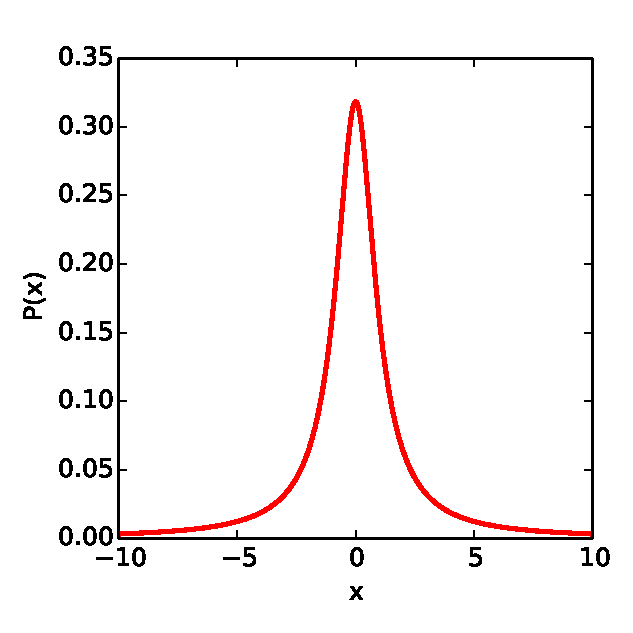
\includegraphics[width=3in]{figures/T_distribution_1df.eps}
	  \caption{t-distribution for one degree of freedom}
\end{figure}

\subsection{Mann-Whitney U Test}\label{sec:mannWhitney}

The Mann Whitney U-test ~\cite{wackerly_mathematical_2007} , also called the Wilcoxon rank-sum test, is a hypothesis test which tests the null hypothesis that one sample has tends to have larger values than another. We begin the Mann Whitney U-test using the same populations, means, and standard deviations as in Welch's t-test. Then we check to see whether or not the following four assumptions are satisfied. 

\begin{enumerate}
	\item $X$ and $Y$ are independent of each other
	\item All observations are ordinal (i.e. it can be distinguished that one observation is greater than another) 
	\item Under the null hypothesis both groups are equal
	\item Under the alternate hypothesis the probability of an observation from one population exceeding an observation from the other is not 0.5. 
\end{enumerate}

In order to perform the test we compute the $U$ statistic.  There are two methods for computing the $U$ statistic: one for small data sets (less than 20 elements) and one for larger data sets.  As all of the datasets used in this are on the order of $10^6$ elements we will only be discussing the latter.

The first step is to rank all the observations. The smallest observation is assigned the rank 1, the next smallest value is assigned the rank 2, and so on.  Ties are equal to the midpoint of the assigned rankings. So in the set $\{2,4,4,7\}$ the ranks $\{1, 2.5, 2.5, 4\}$ would be assigned. 

The next step is to sum the ranks of all observations taken from $X$ and call it $R_1$.  The sum of the ranks from observations taken from $Y$ is given by $R_2$. We can then then compute the $U$ statistics 

\begin{equation}\label{U1}
	U_1=n_1 n_2 + \frac{n_1(n_1+1)}{2} - R_1
\end{equation}

\begin{equation}\label{U2}
	U_2=n_1 n_2 + \frac{n_2(n_2+1)}{2} - R_2
\end{equation}

The smaller of $U_1$and $U_2$ is chosen for computing the p-value which are obtained through a table of critical values. As with the t-test we will be using the scipy implementation ~\cite{jones_scipy:_2001} for our Mann Whitney U-tests. 

\section{Mutual Information}

Mutual information is a quantity which measures the amount of certainty gained about a population $X$ when measuring some random variable $Y$.  In particular let $Y\in {0,1}$ represent whether or not the VM is monitored by some VMI agent and let $X\in \mathbb{R}^n $represent the measured data from a given experiment.  The mutual information   then specifies how many bits of information are gained about $Y$ when sampling the random variable $X$.  Given a joint probability distribution $P(Y=y,X=x)$  the mutual information is given by 

\begin{equation}\label{MutInformEq}
	I(Y:X) = \sum_{x\in X}\sum_{y\in Y} p(y,x)lg(\frac{p(y,x)}{p(x)p(y)})
\end{equation}

To estimate the mutual information, we use the implementation provided by scikit-learn~\cite{pedregosa_scikit-learn:_2011-1} where $X$ is approximated by histograms over a large number of sample measurements. Mutual information will allow us to determine how much many samples are needed in order to make a classification between two samples.
